\documentclass{article}
\usepackage[utf8]{inputenc}
\usepackage{listings} %result code table
\usepackage{hyperref} %link
\usepackage{graphicx} %images
\graphicspath{ {./images/} }


\title{Icosahedron Navigation}
\author{Joel Grayson \& Nathaniel Thornell}
\date{July 3, 2022}

\begin{document}
\maketitle

\section{Problem}
This problem is derived from \href{https://www.janestreet.com/imo2022/}{Jane Street's sample problem for the 2022 International Math Olympiad (janestreet.com/imo2022)}.



\section{Solutions}
\subsection{Method 1}
Method 1 involves marking the starting vertex red. Then, we move to the next vertex and mark it orange as part of the second layer. Layers are sets of vertices that are equidistant from the starting vertex. We then move back to the starting vertex by moving until we reach a red vertex. We can move to any marked vertex by randomly moving around until we reach that marker. We move from the red starting vertex and mark orange, keeping track of how many orange markers we have placed. Once we have placed five orange markers, we move on to placing green markers on the third layer. After marking the three layers, navigate to the vertex without a marker. That unmarked vertex is opposite the red vertex.

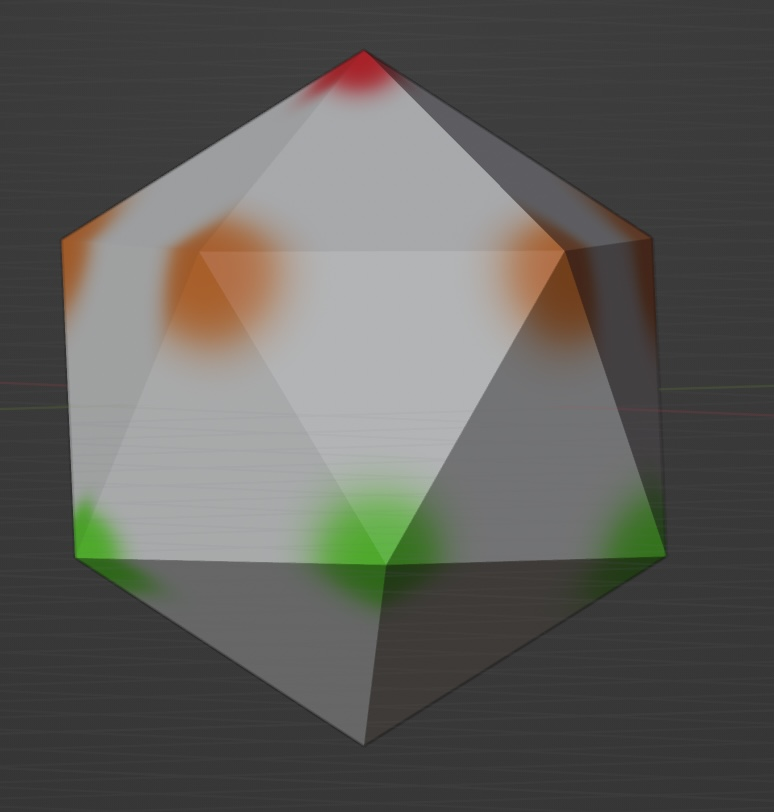
\includegraphics[width=3cm]{model1.jpg}
\caption{The marked icosahedron.}


\subsection{Method 2}
Method 2 is method 1, but with additional rules that save three markers. Since there are an infinite number of colors, we can associate each different color with a meaning. First, we mark the starting spot with a color that means "variable" because we move the marker to a different spot later. Then, we move from the starting vertex and mark that vertex as 2-middle, meaning it the main vertex of the second layer. We then mark the other vertices on the second layer with their own distinct colors by moving back to the start. They are each different colors, so they can be recognizable.

We go to 2-middle and mark the two neighboring vertices without markers as 3-middle and 3-middle-neighbor. We move var (from the starting vertex) to the vertex next to 3-middle on the third layer that is not 3-middle-neighbor.

We go to 3-middle and move once. If that vertex is empty, it is the opposite side. If not, move back to 3-middle and repeat.

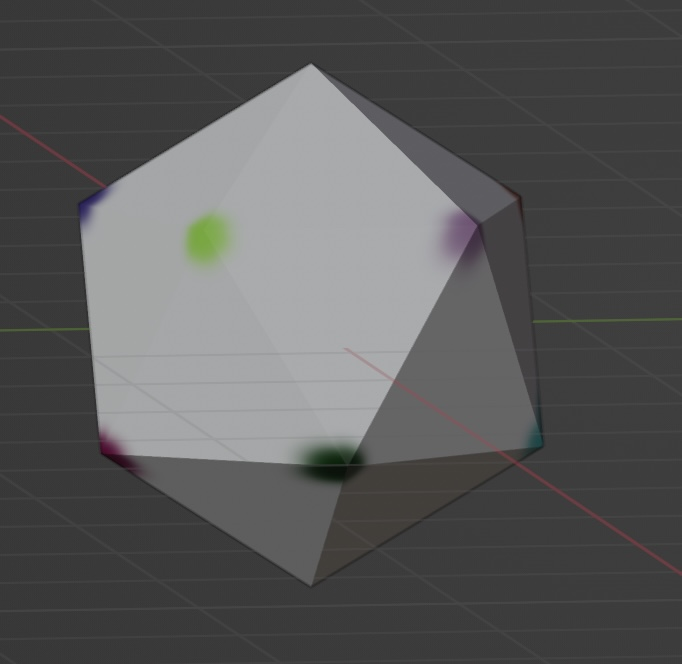
\includegraphics[width=3cm]{model2.jpg}
\caption{Each marker is a unique color, so we can map textual meaning to the colored points.}


\subsection{Method 3}
Mark the starting vertex red. Move three times and mark that vertex green. Then, go back and forth between the red and green vertices a large number of times. If we did not ever travel between the two vertices in fewer than three moves, then it is very likely, but not certain, that you are at the opposite vertex.

In our code, we went back and forth 100 times, leading to a 99.95\% accuracy that you ended up at the opposite vertex. In theory, you would need to go back and forth an infinite number of times to verify for certain. For this reason, we do not consider this solution valid.

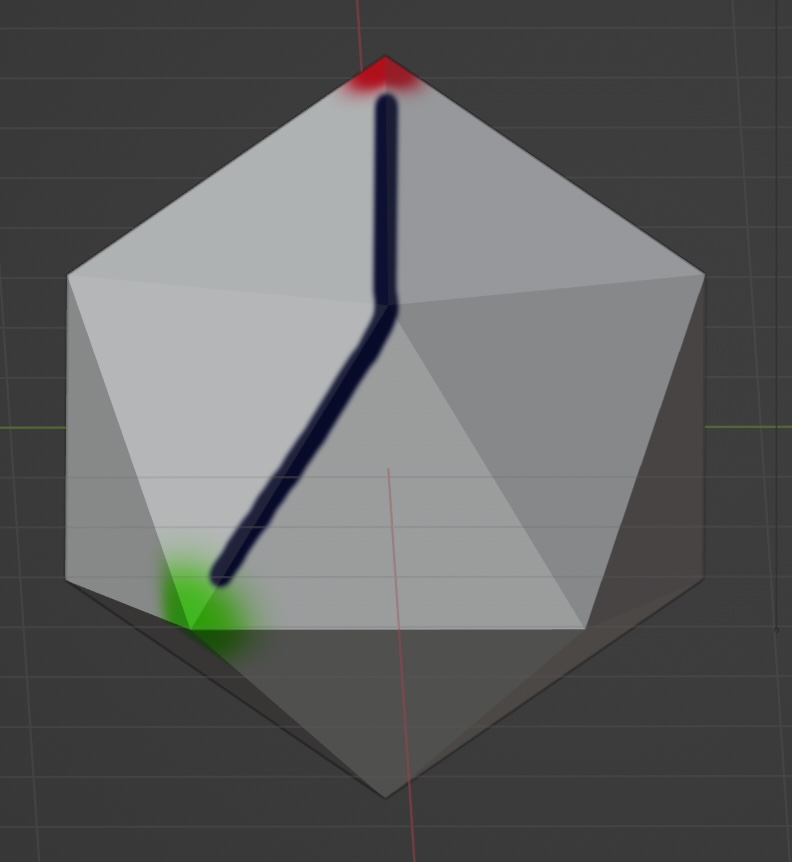
\includegraphics[width=3cm]{model3.jpg}
\caption{Distance between start (red) and end (green) is
two, so green cannot be the opposite side.}

\subsection{Comparison}
Each method has its own advantages:

Method 1 is the easiest to understand as it only uses three colors and takes around two hundred moves to complete. At the end, there is a 100\% guarantee that you're at the opposite side.

Method 2 saves three markers compared to method 1 but is more complicated and confusing. The instructions are harder to explain to someone, there are more marker colors, and it takes more moves.

Once completing methods 1 and 2, there is a 100\% certainty that you are at the opposite vertex. However, method 3 does not have this certainty. Also, method 3 requires a huge number of moves for verification. The benefit is that it only needs two markers.


Here are the average results of running each method 2000 times.
\begin{lstlisting}
|-----------------------------------------------------------|
|                          Results                          |
|                    Method 1      Method 2     Method 3    |
| Accuracy        1.0           1.0          0.9995         |
| Moves           208.078       1625.5525    5068.315       |
| #Total markers  11            8            2              |
| #Unique Markers 3             8            2              |
|-----------------------------------------------------------|
\end{lstlisting}


\end{document}
